% Copyright 2026 Torbjörn E. M. Nordling
% SPDX-License-Identifier: Apache-2.0
% frame-step-10.tex — Step 0.6 to 1.0: another gain and time constant (11:00–12:30)
% Article §3.3: \UpTenGainD, \UpTenTauD, \UpTenDelayD, \GainDrop, \TauRatio,
% \PredOne, \MeasOne.
\begin{frame}{Step 3: 0.6 to 1.0 --- another gain and time constant}{P2 fails}
  \footnotesize
  \begin{columns}[T]
    \column{0.58\textwidth}
    \centering
    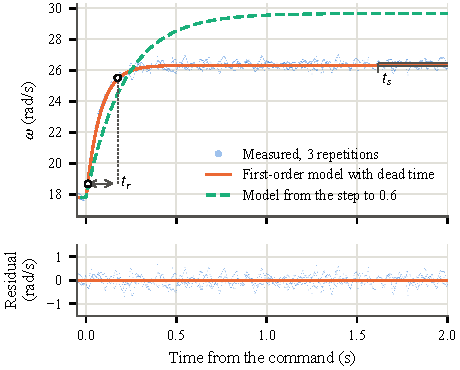
\includegraphics[width=\linewidth, height=0.8\textheight, keepaspectratio]{fig-step-10.pdf}
    \column{0.4\textwidth}
    \scriptsize
    \begin{itemize}\setlength{\itemsep}{3pt}
      \item Fit: $G = \UpTenGainD$\,rad/s, $\tau = \UpTenTauD$\,ms, $\theta = \UpTenDelayD$\,ms.
      \item Gain \alert{\GainDrop\,\% lower}, time constant \alert{\TauRatio{} times shorter} than step 2.
      \item The step-2 model predicts \PredOne\,rad/s at duty 1.0; measured \MeasOne\,rad/s.
      \item \textbf{Causes:} the steady speed is not proportional to the duty, and the driver's fast-decay PWM makes current and damping depend on duty and speed.
    \end{itemize}
  \end{columns}
\end{frame}
